\ifdefined\handoutmode
  \PassOptionsToClass{handout}{beamer}
\fi
\documentclass[aspectratio=169]{beamer}

\input{../../../../hh_bpa_forel-preamble} % this is ugly.

\title{FMTS mätteknik HT2026 -- Dag 3}
\author{Pererik Andreasson \\ Struan Gray }
\date{\today{}}

\begin{document}

%%% Title slide: different footer, large logo
{
% no page #, no logo on title page
\setbeamertemplate{footline}{}
\setbeamertemplate{logo}{\titlelogos}
\begin{frame}
\vfill
  \begin{block}
    \maketitle
  \end{block}
\end{frame}
}


\frame{
    \frametitle{Lärandemål}
    {\Huge
    \begin{enumerate}
        \item<1-> Ensam mätning inget värt.
        \item<2-> Okalibrerat mätinstrument inget värt.
        \item<3-> Elektriska mätningar \emph{påverkar} mätobjektet $\rightarrow$ behöver \emph{tolkas}.
    \end{enumerate}
    }
}


\mode<beamer>{
\frame{
    \frametitle{Dagens plan}
    {\Large
        \begin{itemize}
            \item AC - växelström.
            \item RMS vs. True RMS.
            \item Oscilloskopmätningar.
            \item Halvledare -- dioder.
            \item Likriktare.
        \end{itemize}
    }
    }   
} % end mode


\mode<beamer>{
%%--------------
%% Ny frame
%%--------------
\begin{frame}{Hur gick det igår med tidskonstanten?}
    \begin{columns}
        \column{0.2\textwidth}
  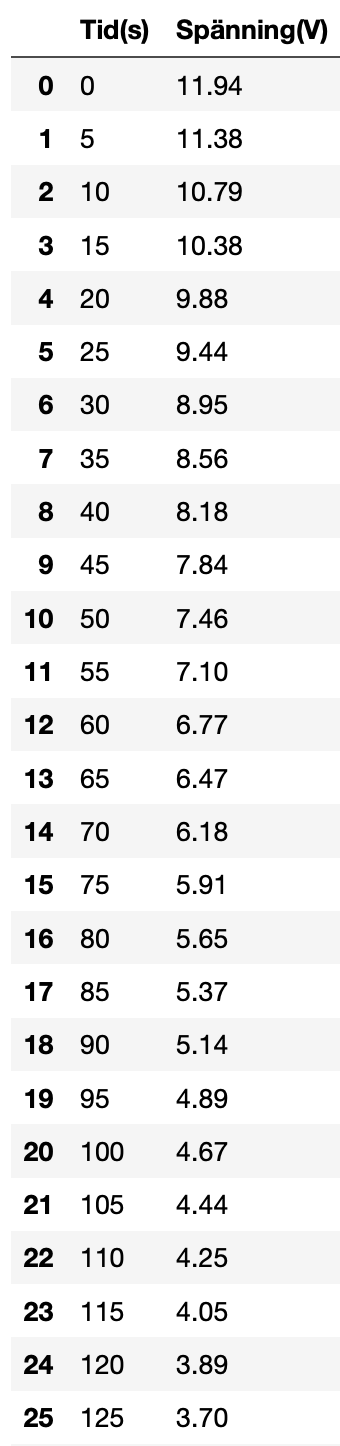
\includegraphics[height=0.8\textheight]{figures/kond_tabell.png}
        \column{0.8\textwidth}% <2->
  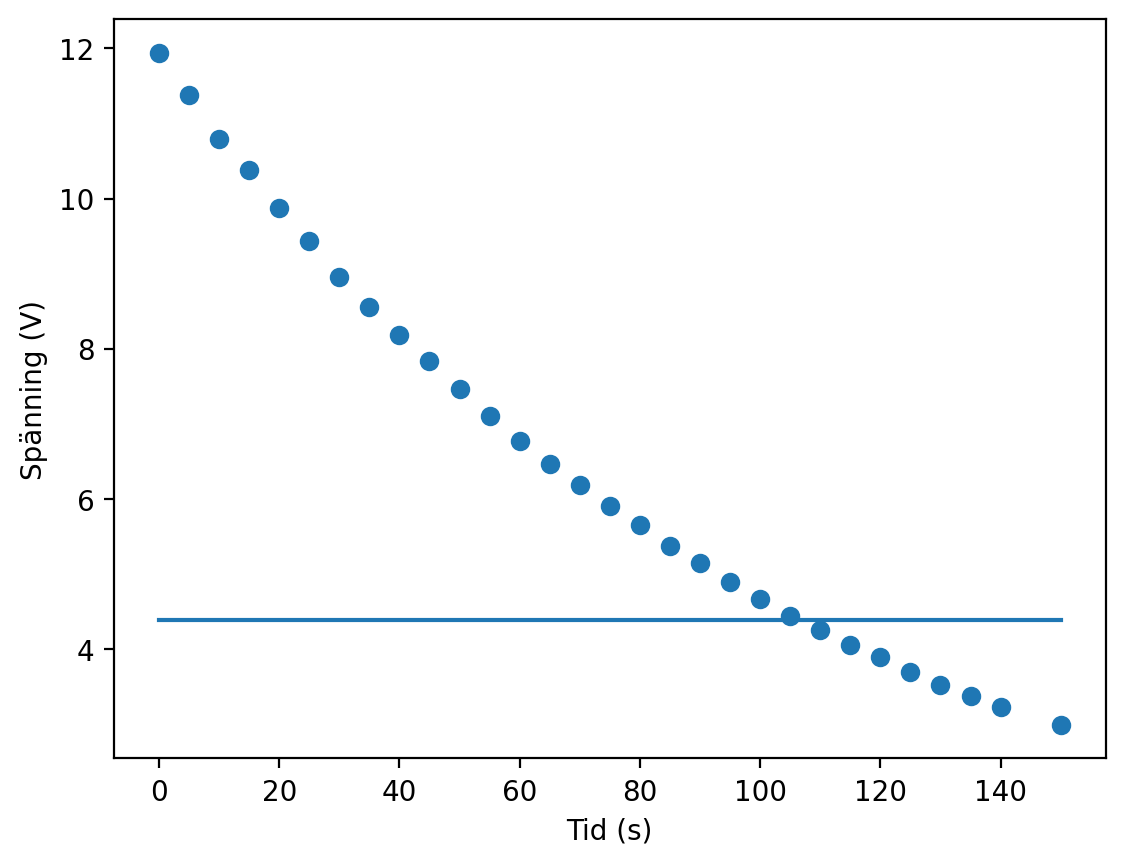
\includegraphics[width=0.7\textwidth]{figures/konding_labb.png}
    \end{columns}
\end{frame}
} % end mode


\mode<beamer>{
\frame{
\frametitle{}
{\Huge Växelström och likström}
}
} % end mode




%%--------------------------------------------------
%% Ny frame - amplitud och frekvensbilden
%%--------------------------------------------------
\begin{frame}<7>[fragile]{Växelström och växelspänning}
	\resizebox{0.8\textwidth}{!}{
  \begin{tikzpicture}[scale=1.5]
	\datavisualization [scientific axes, visualize as smooth line,
						x axis={label=Tid (\unit{\micro\s}), ticks={
						major={at={0,90,180,270,360}}}},y axis={
						label=Spänning (\unit{\mV}), ticks={
						major={at={-1, -0.75,-0.5,-0.25,0,0.25,0.5,0.75,1}}}}]
		data [format=function] {
			var x : interval [-5:365];
			func y = sin( \value x );
			};
		\onslide<2->{
		% amplitudoverlay
		\draw (1.5,2.32) node[anchor = west, red] 
		{Amplitud, $\hat{u}=\qty{1}{\mV}$} ;
		\draw[red, very thick, |-|] (1.285,1.55) -- (1.285, 3.09) ;	
		}
		\onslide<3->{
		% Periodtidoverlay
		\draw[blue, very thick, |-|] (0.06,1.545) -- (4.94, 1.545) ;
		\draw (0,1.25) node[anchor = west, blue] {Periodtid, 
		$T=\frac{1}{f}=\qty{360}{\us}$} ;}
        \onslide<4->{
        \draw (3, 1.25) node[anchor = west, blue] {$\Rightarrow f\approx\qty{2.78}{\kHz}$} ;
        }
        \onslide<5->{
		\draw (0, 0.75) node[anchor = west, blue] {Vinkelfrekvens, $\omega = 2 \pi f$} ;
        }
        \onslide<6->{
        \draw (2.75 , 0.75) node[anchor = west, blue] {$\approx\qty{17.4}{\kilo\radian\per\s}$};
        }
      \onslide<7->{
        \draw[ultra thick, <->] (5, 0) -- (5, 3.1) node[midway, below, rotate=90] {PeakToPeak} ;
      }
	\end{tikzpicture}
  } % End resizebox
  \\[-5mm]
	\onslide<7->{
    {\Large
	\[ u(t) = \qty{1}{\mV} \sin \big( \qty{17.4}{\kilo\radian\per\s} t \big) \]
    }
	}
%\end{columns}
\end{frame}


\handoutnoteslide


%%--------------------------------------------------
%% Ny frame
%%--------------------------------------------------
\begin{frame}[fragile]{Växelström - Kondensatorn}
	
	{\LARGE
	Över en kondensator med kapacitansen \qty{470}{\uF} ligger  en sinusformad spänning som har amplituden \qty{2}{\V} och frekvensen \qty{1000}{\Hz}. 
  \begin{enumerate}
    \item Beräkna kondensatorns reaktans.
    \item Beräkna amplituden hos strömmen genom
	kondensatorn.
    \item Beräkna spänningen vid tiden \qty{0.5}{\ms}.
  \end{enumerate}
  
	} % end LARGE
\end{frame}


\handoutnoteslide


%%----------------
%% Ny frame
%%----------------
\begin{frame}[fragile]{Växelströmsmätning -- effektivvärde}
  \begin{columns}
    \column{0.1\textwidth}
        \begin{circuitikz}[american]
            \draw (0, 0) to[R=$R$, v=$u(t)$] (0, 2);
        \end{circuitikz}
    \column{0.45\textwidth}<2->
          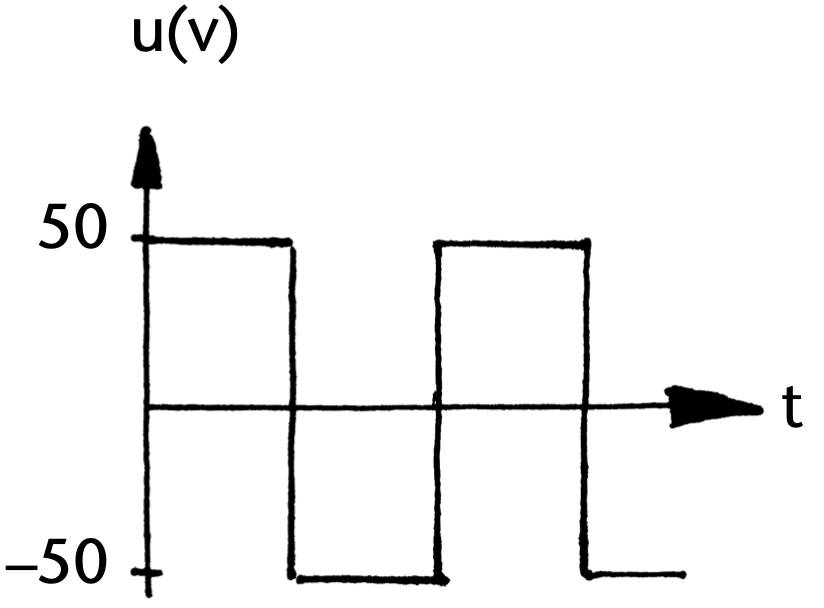
\includegraphics[width
          =0.9\textwidth]{figures/effektivvarde_fyrkant.png}\\
    \column{0.45\textwidth}<5->
          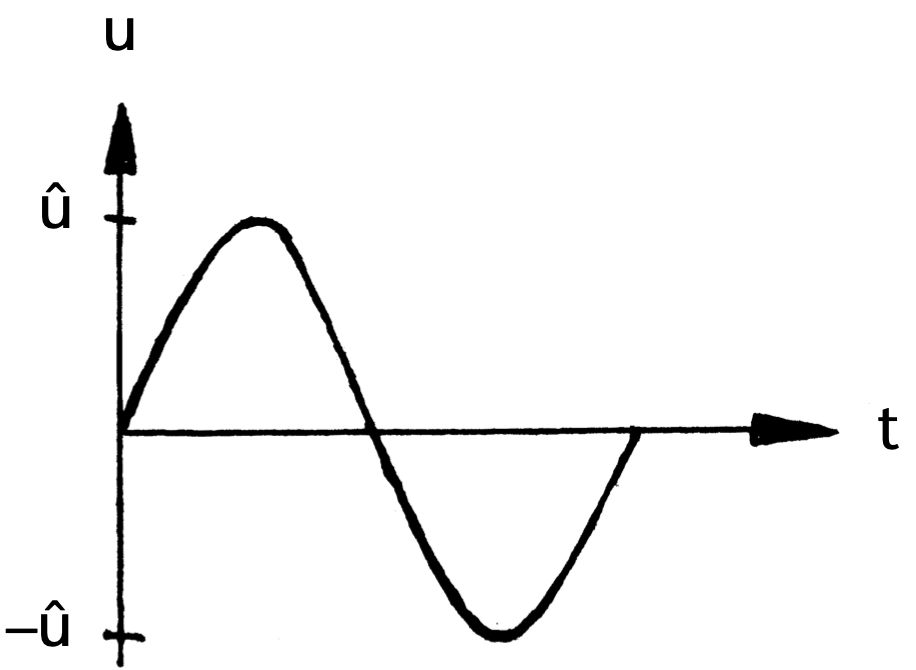
\includegraphics[width
          =0.9\textwidth]{figures/effektivvarde_sinus.png}\\
        \end{columns}
        {\LARGE
        \begin{itemize}
        \item<2-> Fyrkant: \emph{amplitud} $\hat{u}=\qty{50}{\volt}$
          Effektutveckling?
          \item<3-> Som likspänning: \onslide<4->{
              \emph{effektivvärdet} är $u_\mathrm{eff}=\hat{u}=\qty{50}{\volt}$ }
          
        \item<5-> Sinus: $u(t)=\hat{u}\sin\omega t$ \onslide<6->
          Vilken DC ger samma $P$ i $R$?
        \item<7-> $P=UI=\frac{U^2}{R} \hspace{5mm} \pause{} \Rightarrow$ \hspace{5mm} $p(t)=\frac{\hat{u}^2\sin^2\omega t}{R}$
	\end{itemize}
        } % large ends
\end{frame}


\handoutnoteslide


\mode<beamer>{
  \sectionslide{Vet alla \alert{väl} vad $\sin x$ betyder?}
}

\begin{frame}{\(\sin x\)}
    \centering
    \resizebox{0.75\textwidth}{!}{
    \begin{tikzpicture}[
        line width=1.2pt,
        every node/.style={font=\Large}
    ]
        \coordinate (A) at (0,0);
        \coordinate (B) at (6,0);
        \coordinate (C) at (6,3.5);

        \draw (A) -- (B)
                  -- node[right] {$a$} (C)
                  -- node[above left] {$c$} (A);

        % Right angle and angle x
        \pic[draw, angle radius=0.35cm]
            {right angle=A--B--C};
        \pic[draw, "$x$", angle radius=1.1cm, angle eccentricity=1.3]
            {angle=B--A--C};
    \end{tikzpicture}
    } % end resizebox
    \pause{}
    \bigskip
    {\LARGE \(\displaystyle \sin x=\frac{a}{c}\)}
\end{frame}

\handoutnoteslide


\begin{frame}{The unit circle -- Om $x$ ökar, vad händer då?}
    \centering
    \resizebox{0.6\textwidth}{!}{
    \begin{tikzpicture}[
        scale=2.3,
        line width=1.2pt,
        every node/.style={font=\large}
    ]
        % Same triangle proportions as before
        \pgfmathsetmacro{\ang}{atan(3.5/6)}

        \coordinate (O) at (0,0);
        \coordinate (P) at (\ang:1);
        \coordinate (B) at ({cos(\ang)},0);

        % Coordinate axes and unit circle
        \draw[->, thin, gray] (-1.25,0) -- (1.3,0);
        \draw[->, thin, gray] (0,-1.2) -- (0,1.25);
        \draw (O) circle[radius=1];

        \node[below left] at (O) {$0$};
        \node[below right] at (1,0) {$1$};
        \node[above left] at (0,1) {$1$};

        % Inscribed right triangle
        \draw (O) -- (B)
                  -- node[right] {$\sin x$} (P)
                  -- node[above left] {$1$} (O);

        \pic[draw, angle radius=0.18cm]
            {right angle=O--B--P};
        \pic[draw, "$x$", angle radius=0.7cm,
             angle eccentricity=1.35]
            {angle=B--O--P};

        \fill (P) circle[radius=0.025];
    \end{tikzpicture}
    } % end resizebox
\end{frame}

\handoutnoteslide

\mode<beamer>{
\begin{frame}{One period of a sine wave}
    \centering
    \begin{tikzpicture}
        \begin{axis}[
            width=0.95\textwidth,
            height=0.8\textheight,
            xmin=0, xmax=2*pi,
            ymin=-1.2, ymax=1.2,
            axis lines=middle,
            xlabel={$x$},
            ylabel={$\sin x$},
            %xtick={0,1.570796,3.141593,4.712389,6.283185},
            %xticklabels={
            %    $0$,$\frac{\pi}{2}$,$\pi$,
            %    $\frac{3\pi}{2}$,$2\pi$
            %},
            ytick={-1,1},
            tick label style={font=\large},
            label style={font=\Large},
            axis line style={thick},
            grid=major,
            grid style={gray!25},
        ]
            % Expand the step number before PGFPlots stores the plot.
            \foreach \step in {1,...,20}{
    \edef\drawsegment{%
        \noexpand\addplot[
            black,
            line width=1.8pt,
            visible on=<\step->,
            domain={(\step-1)*pi/10}:{\step*pi/10},
            samples=21
        ] {sin(deg(x))};
    }
    \drawsegment
}
        \end{axis}
    \end{tikzpicture}
\end{frame}
} % end mode



% One Beamer slide:
\begin{frame}{Sinusoidal voltage and instantaneous power}
    \centering
  \(u(t)=\qty{10}{\V}\sin(100\cdot 2\pi t),
      \qquad R=\qty{50}{\ohm},
      \qquad p(t)=\dfrac{u^2(t)}{R}\)

    \medskip
    \begin{tikzpicture}
        \pgfplotsset{
            presentation axis/.style={
                width=0.8\textwidth,
                height=0.65\textheight,
                scale only axis,
                xmin=0, xmax=10,
                domain=0:10,
                samples=401,
                axis line style={black, thick},
                tick style={black, thick},
                tick align=outside,
                tick label style={font=\large},
                label style={font=\large},
                scaled ticks=false,
            }
        }

        % Voltage: left axis. The horizontal variable is time in ms.
        \begin{axis}[
            presentation axis,
            ymin=-12, ymax=12,
            axis y line*=left,
            axis x line*=bottom,
            xlabel={Time (ms)},
            ylabel={Voltage (V)},
            xtick={0,2,4,6,8,10},
            ytick={-10,-5,0,5,10},
            grid=major,
            grid style={gray!25},
        ]
            % pgfplots evaluates trigonometric functions in degrees.
            \addplot[black, line width=1.6pt]
                {10*sin(36*x)};

            \draw[gray!60, thin]
                (axis cs:0,0) -- (axis cs:10,0);
        \end{axis}
  \begin{scope}[visible on=<2->]
        % Instantaneous power: right axis.
        \begin{axis}[red, 
            presentation axis,
            ymin=0, ymax=2.4,
            axis y line*=right,
            axis x line=none,
            ylabel={Power (W)},
            ytick={0,0.5,1,1.5,2},
        ]
            \addplot[red, dashed, line width=1.6pt]
                {(10*sin(36*x))^2/50};
        \end{axis}
      \end{scope}
    \end{tikzpicture}
\end{frame}

\handoutnoteslide

%%--------------------------------------------------
%% Ny frame
%%--------------------------------------------------
\begin{frame}[fragile]{Växelströmsmätning -- effektivvärde}
  \begin{columns}
    \column{0.1\textwidth}
        \begin{circuitikz}[american]
            \draw (0, 0) to[R=$R$, v=$u(t)$] (0, 2);
        \end{circuitikz}
    \column{0.45\textwidth}
          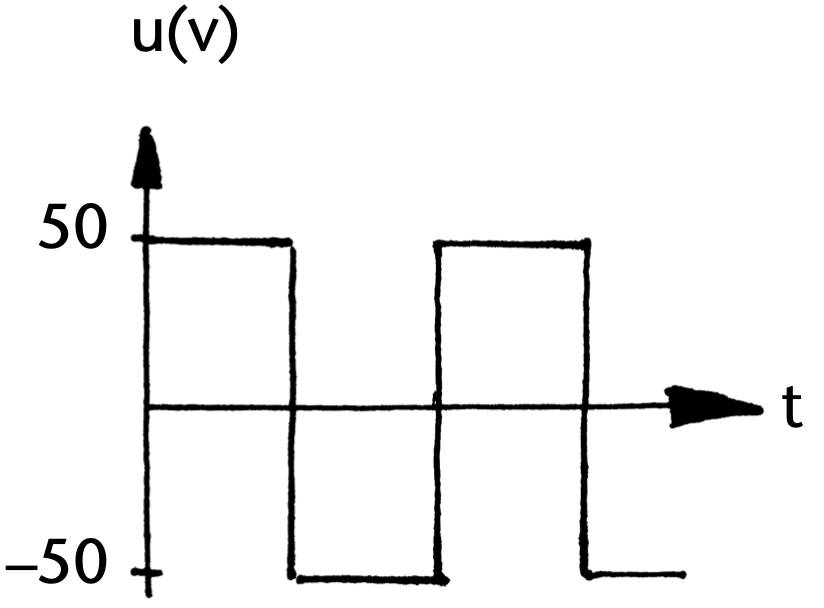
\includegraphics[width
          =0.9\textwidth]{figures/effektivvarde_fyrkant.png}\\
    \column{0.45\textwidth}
          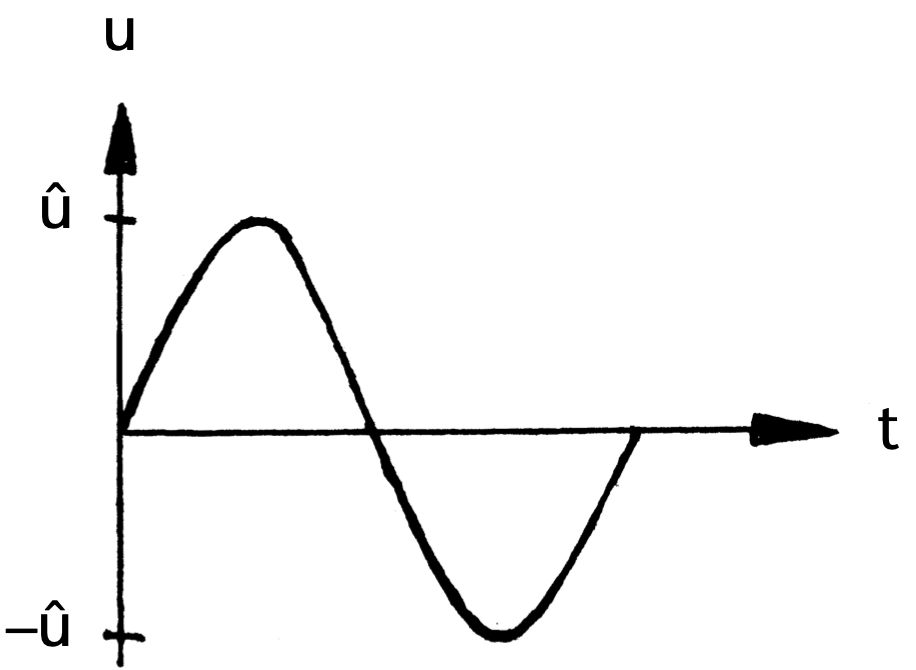
\includegraphics[width
          =0.9\textwidth]{figures/effektivvarde_sinus.png}\\
        \end{columns}
\begin{center}
{\LARGE
\onslide<2->{Effektiva spänningen blir:}
\onslide<2->{$u_\mathrm{eff}=\frac{\hat{u}}{\sqrt{2}}$}
\onslide<2->{för \alert{sinus}-signaler.}\\
\onslide<3->{$u_\mathrm{eff}=u_\mathrm{RMS}=$}
\onslide<3->{\emph{Root Mean Square}}
}  
\end{center}
\end{frame}

\handoutnoteslide

%% --------------------------------------------------
%% Ny frame
%%--------------------------------------------------

\begin{frame}[fragile]{RMS-värden -- exempel}
  \begin{columns}
    \column{0.5\textwidth}
          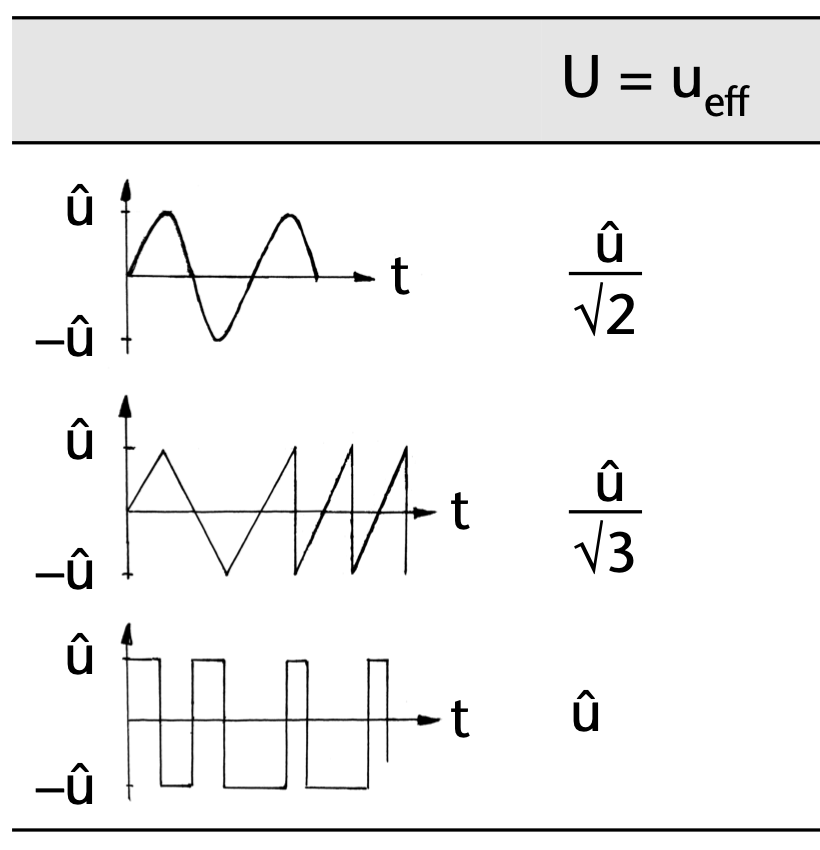
\includegraphics[width
          =\textwidth]{figures/rmstabell.png}\\
    \column{0.5\textwidth}<2->
          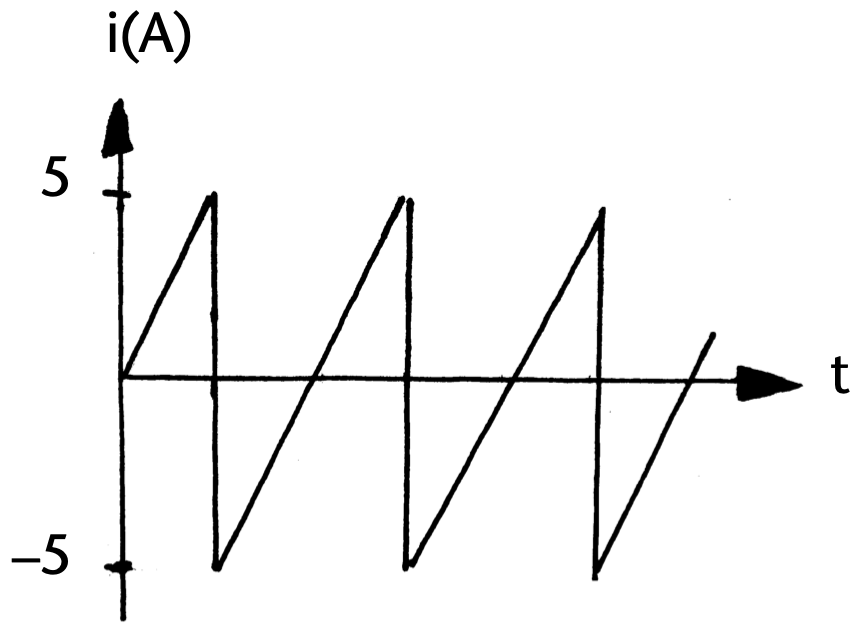
\includegraphics[width
          =\textwidth]{figures/sagtand.png}\\
          \onslide<3->{Vilken effekt utvecklas av strömmen oven i ett \qty{10}{\ohm}-motstånd?}
        \end{columns}
\end{frame}


\handoutnoteslide

%% --------------------------------------------------
%% Ny frame
%%--------------------------------------------------

\begin{frame}[fragile]{Multimetrar}

  RMS-värden visas av multimetrar vid AC-mätning -- \alert{men hur fås dessa?}
  \begin{columns}
    \column{0.67\textwidth}<2->
          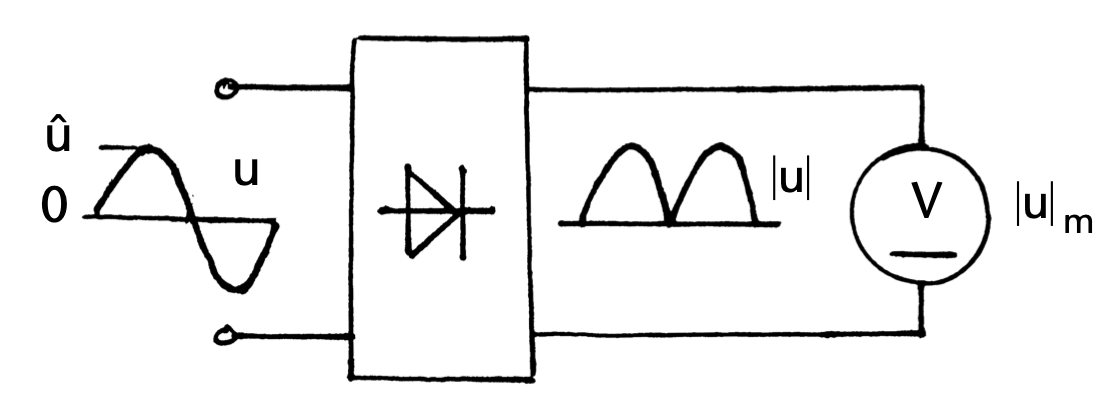
\includegraphics[width
          =\textwidth]{figures/multilikriktare.png}\\
    \column{0.33\textwidth}<3->
          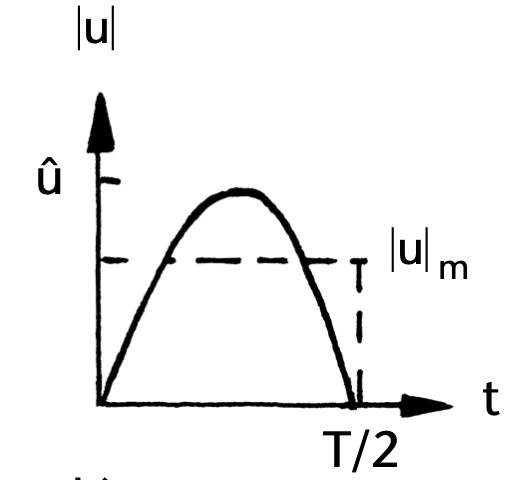
\includegraphics[width
          =\textwidth]{figures/multilikriktaresignal.png}\\
        \end{columns}
{\LARGE
    \begin{center}
    \onslide<3->{Effektivvärdet är \num{1.11} ggr större, dvs $u_\mathrm{RMS}=1.11\cdot{}|u|_m$
    }

  \onslide<4->{ RMS-mutlimetrar visar rätt för \alert{sinus}-signaler
    med medelvärdet noll $\Rightarrow$ annars fel!\\
  }
\end{center}
} % end LARGE
\end{frame}

\handoutnoteslide

% bnc kontakter genomgång
%% BNC och koaxialkablar
\mode<beamer>{
\sectionslide{Koaxialkablar och BNC-kontakter}
} % end mode

\descriptionslide{figures/coaxial-cable.png}{1}{Koaxialkabel}{}

\handoutnoteslide

\descriptionslide{figures/bnc_stift_v2.png}{0.5}{BNC-stift: sitter på kabeln.}{}

\descriptionslide{figures/bnc_hylsa_v2.png}{0.5}{BNC-hylsa: sitter på instrumentet. (eller på olika adaptrar.)}{}

\descriptionslide{figures/bnc_anslutning.png}{0.5}{BNC-anslutning}{}

\instructionslide{Öva på att ansluta BNC-kontakter med T-korsen som har delats ut (eller håller på att delas ut).}

\descriptionslide{figures/funktions-koaxial-skop.jpg}{1}{Koppla ihop funktionsgeneratorn (Siglent) och oscilloskopet (Rohde\&Schwarz) med en koaxialkabel.}{}

\handoutnoteslide

\descriptionslide{figures/siglent.png}{1}{Siglent-funktionsgeneratorn.}{}
\handoutnoteslide

% siglent generatorn


\frame{
\frametitle{RMS vs. True RMS}
Koppla upp
\resizebox{0.67\textwidth} {!}{
\begin{tikzpicture}
    \draw (0, 0) to[sinusoidal voltage source] (0, 2) 
    -- (1.5, 2)
    to[R=\qty{50}{\ohm}, *-*] (1.5, 0)
    -- (0, 0);
    \draw (1.5, 2) -- (3, 2)
    to[voltmeter] (3, 0) -- (1.5, 0) ;
\end{tikzpicture}}\\[5mm]
Ställ in funktionsgeneratorn på sågtandssignal, \qty{2}{\V} och \qty{50}{\Hz}.
Växla mellan True RMS och bara RMS (krävs olika multimetrar för detta). Mät AC-spänning. Hur stor är skillnaden?
}
\handoutnoteslide

\begin{frame}{Seriekopplade komponenter.}
$C\approx\qty{64}{\micro\farad}$ och behåll samma motstånd. Koppla  enligt schemat nedan. Använd signalgeneratorns utgång som spänningskälla (AC - sinus). Mät $U_R$ och $U_C$ med multimetern. 
  \begin{center}
\resizebox{0.6\textwidth}{!}{
\begin{tikzpicture}[american]
	\draw (0, 0) node[ground, rotate=-90] {} to[sV, v<=\qty{2}{V}, *-] (4, 0)
		to[short] (4, 2)
		to[C, v=$U_C$] (2, 2)
		to[R, v=$U_R$] (0, 2)
		to[short] (0, 0) ;
\end{tikzpicture}
} % end resizebox
\end{center}
\end{frame}

\handoutnoteslide

% det finns en triggering bild på bilder05-slidesen. 
% fundera på om den skall vara här och om det skall vara
% en explicit övning. 

\mode<beamer>{
\descriptionslide{figures/gammalt_oscilloskop.png}{0.9}{Gammalt oscilloskop}{}

\descriptionslide{figures/crt-teknik.png}{1}{Gammal teknik -- elektronstråle sveps.}{}
}

\descriptionslide{figures/rtbskopet.png}{0.8}{RTB oscilloscope}{}

\handoutnoteslide

\begin{frame}{Principskiss oscilloskop}
      \resizebox{1\linewidth}{!}{
        \begin{tikzpicture}[>=latex, font=\sffamily]

            % Signal in
            \node at (1.75,1.21) {Signal};

            % Arrow to amplifier signal
            \draw[thick] (2.2,0.4) circle [radius=0.1];
            \draw[thick] (2.3,0.4) -- (3,0.4);
            \node[anchor=east] at (2,0.4) {Ch$1$};

            % Arrow to amplifier ground
            \draw[thick] (2.2,-0.4) -- (3,-0.4);
            \draw node[anchor=east] at (2,-0.4) {GND};
            \draw[thick] node[ground] at (2.2,-0.4) {};

            % Amplifier triangle
            \draw[thick] (3,0.65) -- (3,-0.65) -- (4.25,0) -- cycle;
            \node at (3.65,1.25) {Förstärkare};

            % Arrow to ADC
            \draw[->, thick] (4.25,0) -- (4.75,0);

            % ADC block
            \node[draw, minimum width=1.5cm, minimum height=1.5cm, thick] (adc) at (5.5,0) {};
            \node at (5.5,1.25) {ADC};

            % parallel bus
            \foreach \y in {-0.15, 0.1}
            \draw[thick] (6.25,\y) -- (7,\y);

            % µ‑dator block
            \node[draw, minimum width=1.5cm, minimum height=1.5cm, thick] (cpu) at (7.75,0) {};
            \node at (7.75,1.25) {\parbox{1.45cm}{\centering Dator \&\\minne}};

            % bus to display
            \foreach \y in {-0.15, 0.1}
            \draw[thick] (8.5,\y) -- (9.0,\y);

            % Display block
            \node[draw, minimum width=2cm, minimum height=1.5cm, thick, anchor=west] (disp) at (9,0) {};
            \node at (10,1.25) {Skärm};

            % Display waveform
            \begin{scope}[shift={(9.25,0)}]
                \draw[thick] plot[domain=0:pi, samples=80] ({0.45*\x},{0.4*sin(5*\x r)});
            \end{scope}
        \end{tikzpicture}
    } % Resizebox

\end{frame}

\handoutnoteslide

\begin{frame}
  \frametitle{Kondensator och oscilloskop}
$C=\qty{100}{\nano\farad}$ och $R=\qty{1}{\kilo\ohm}$. Koppla  enligt schemat nedan. Använd signalgeneratorns utgång som spänningskälla (AC - sinus), se till så kondensatorns reaktans är ungefär lika stor som motståndets resistans! Koppla in oscilloskopens kanaler som visas.
  \begin{center}
\resizebox{0.6\textwidth}{!}{
\begin{tikzpicture}[american]
	\draw (0, 0) node[ground, rotate=-90] {} to[sV, v<=\qty{2}{V}, *-] (4, 0)
		to[short] (4, 2) node[above, yshift=2ex] {Ch1}
		to[C, v=$U_C$] (2, 2) node[above, yshift=2ex] {Ch2}
		to[R, v=$U_R$] (0, 2)
		to[short] (0, 0) ;
\end{tikzpicture}
} % end resizebox
\end{center}
\end{frame}


\handoutnoteslide

% below because the values are NOT good as an example of the time constant, so I commented it out. Better version is in dag04.
% \begin{frame}
% \frametitle{Kondensator och oscilloskop}
% $C=\qty{100}{\nano\farad}$ och $R=\qty{1}{\kilo\ohm}$. Koppla enligt schemat nedan. Använd fyrkantspuler med korta intervall och mät (på oscilloskopet) upp tidskonstanten. Använd markörer eller annan lämplig mätning.
%   \begin{center}
% \resizebox{0.6\textwidth}{!}{
% \begin{tikzpicture}[american]
% 	\draw (0, 0) node[ground, rotate=-90] {} to[sV, v<=\qty{2}{V}, *-] (4, 0)
% 		to[short] (4, 2) node[above, yshift=2ex] {Ch1}
% 		to[C, v=$U_C$] (2, 2) node[above, yshift=2ex] {Ch2}
% 		to[R, v=$U_R$] (0, 2)
% 		to[short] (0, 0) ;
% \end{tikzpicture}
% } % end resizebox
% \end{center}
% \end{frame}

% \handoutnoteslide

\frame{
\frametitle{Nu lite elektronik!}
\resizebox{\textwidth}{!}{%
\begin{minipage}{.5\textwidth}
\centering
  \begin{circuitikz}[american] 
  	\draw (0, 0)  
	to[diode, v=$U_D$] (2, 0)
	;
  \end{circuitikz}
\end{minipage}
}
\\\vspace{1mm}
{\Large  
 Dioden leder bara ström åt ett håll!\\\vspace{1mm}  Ofta $U_D=\qty{0.7}{\V}$
\\\vspace{1mm} 
}
  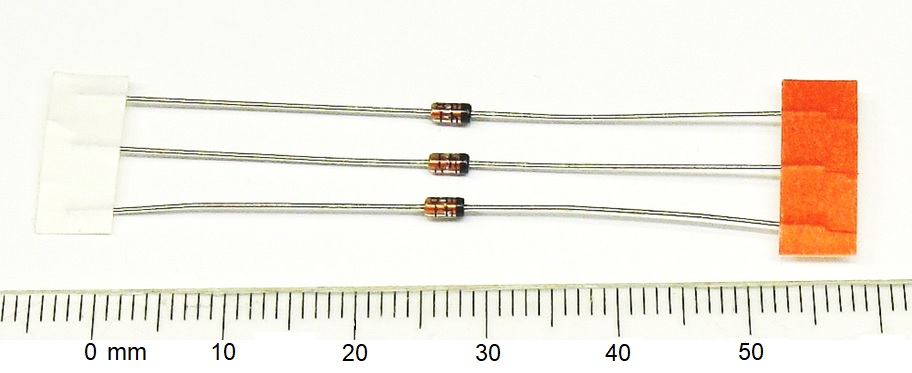
\includegraphics[width = \textwidth]{figures/dioder.jpg}
}

\handoutnoteslide

\frame{
\frametitle{}
\resizebox{0.67\textwidth}{!}{%
\centering
  \begin{circuitikz}[american] 
  	\draw (0, 0)  
    to[sinusoidal voltage source, invert, l=$U$, *-] (0,2)
    to[diode] (2, 2)
    to[R=$R$] (2, 0)
	-- (0, 0)
    node[ground, rotate=-90]{}
    ;
    \draw (2, 2)
    to[short,*-] (4, 2)
    to[oscope] (4, 0)
    to[short, -*] (2, 0) 
    ;
  \end{circuitikz}
} % end resizebox
\\\vspace{3mm}
{\Large  
 Hur ser spänningen över motståndet ut?
\\\vspace{1mm} 
}% end LARGE
} % end frame

\handoutnoteslide

\mode<beamer>{
\frame{
    \frametitle{}
    \begin{tikzpicture}[remember picture,overlay]
        \node[at=(current page.center)] {
            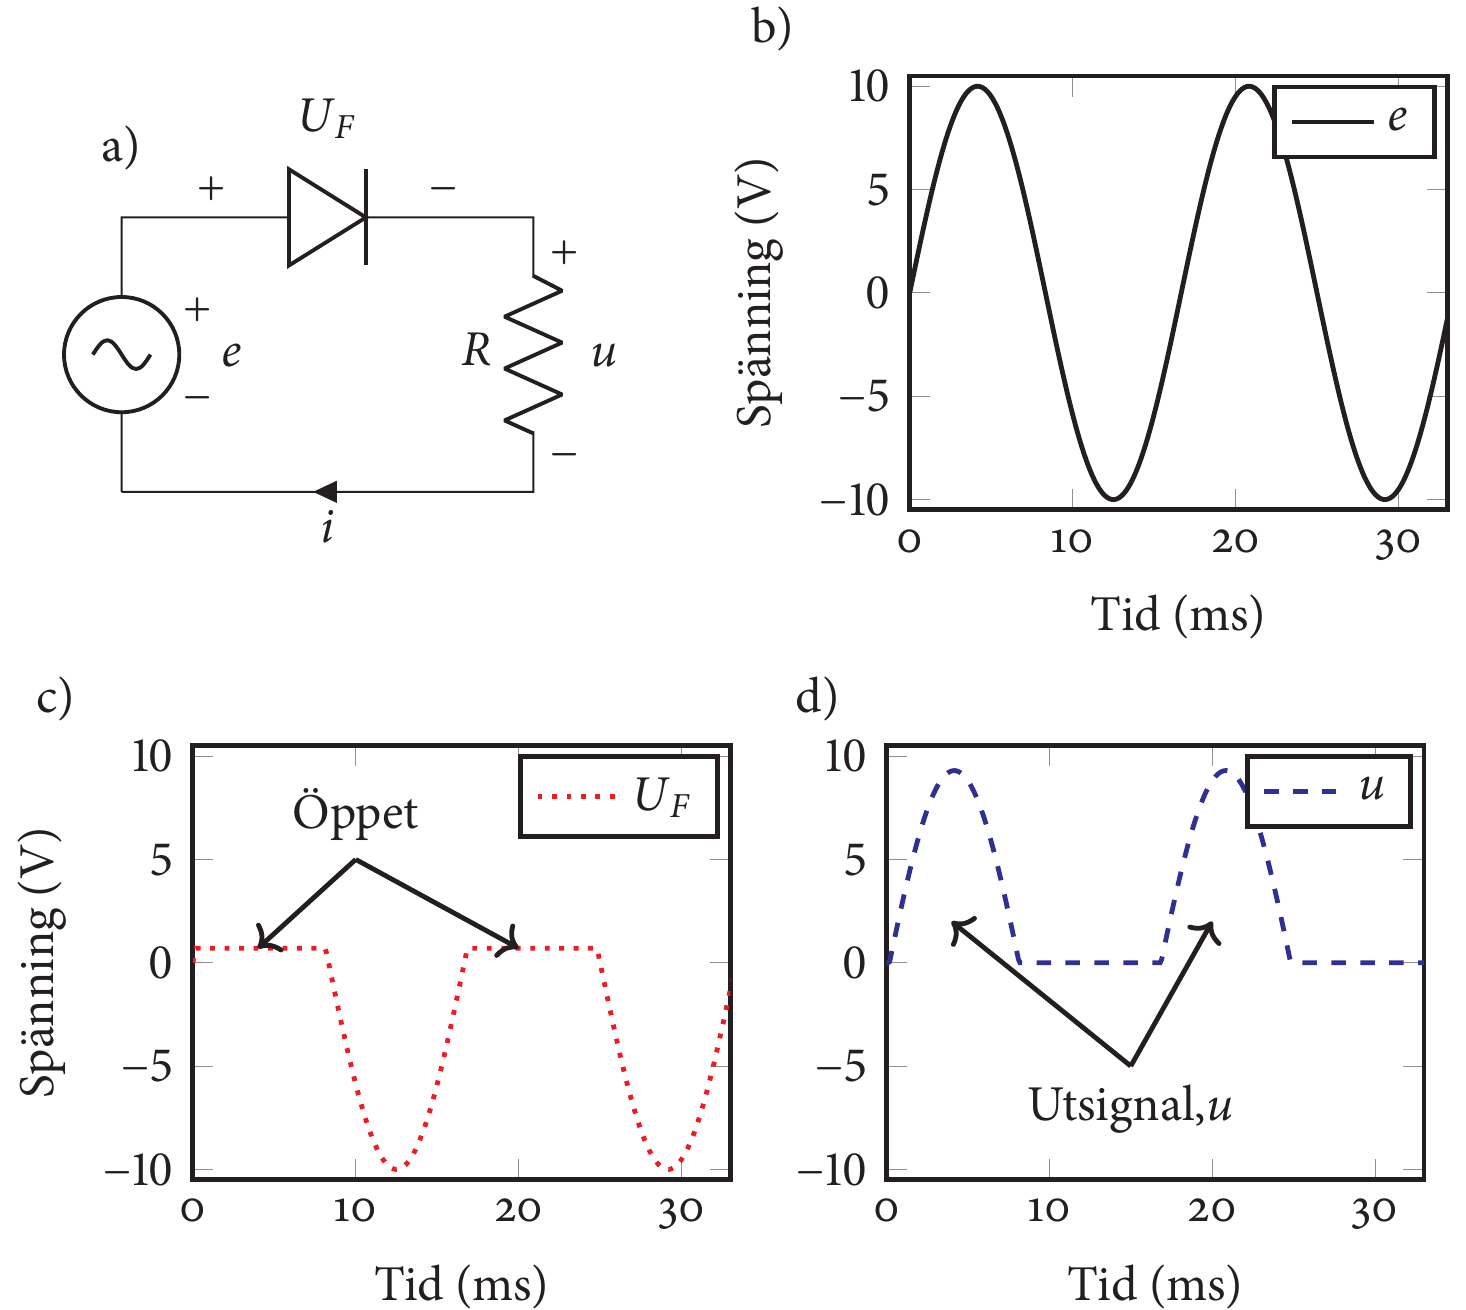
\includegraphics[keepaspectratio,
                                 width=\paperwidth,
                                 height=\paperheight]{figures/diod_svaret.png}
            };
    \end{tikzpicture}    
  }
}

\frame{
\frametitle{}
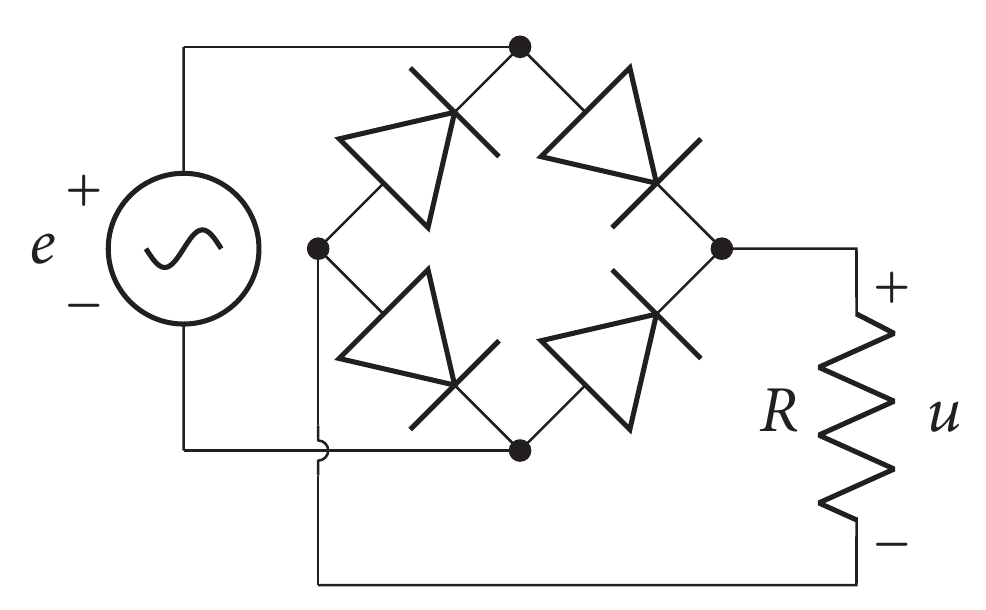
\includegraphics[width=\textwidth]{figures/likriktare.png}
}

\handoutnoteslide

\mode<beamer>{
\frame{
\frametitle{}\centering
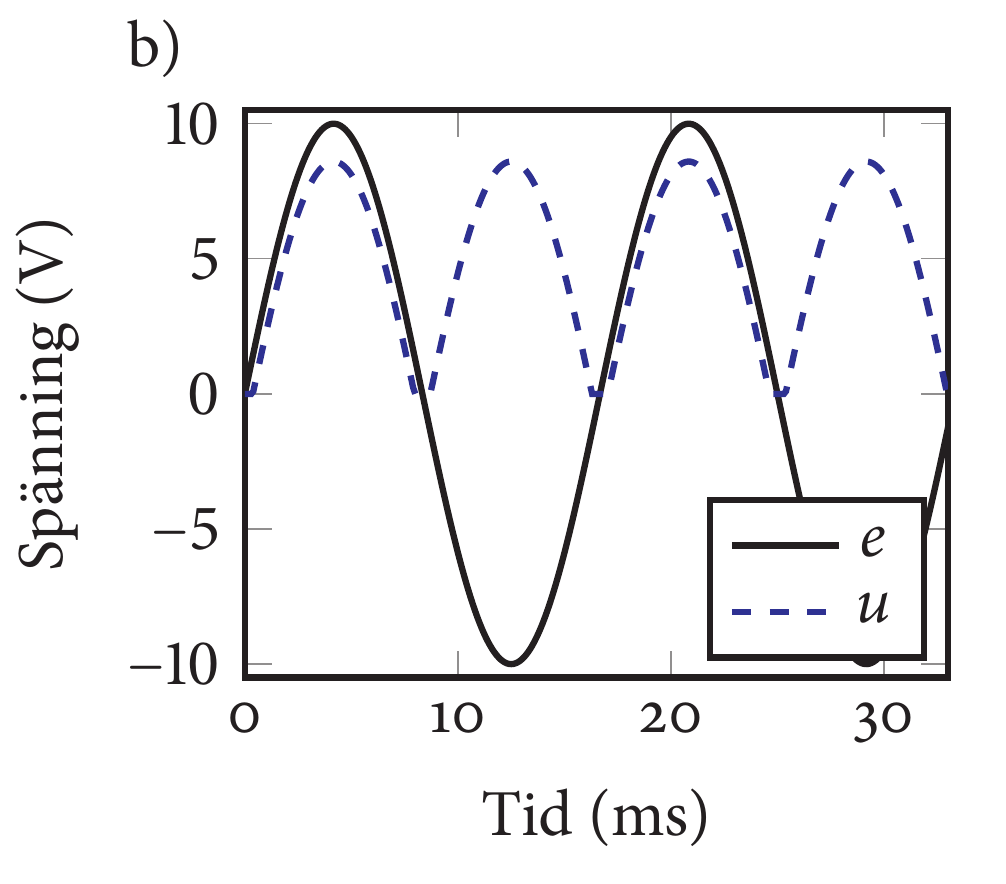
\includegraphics[width=0.7\textwidth]{figures/likriktare_svaret.png}
}
} 

\frame{
\frametitle{}
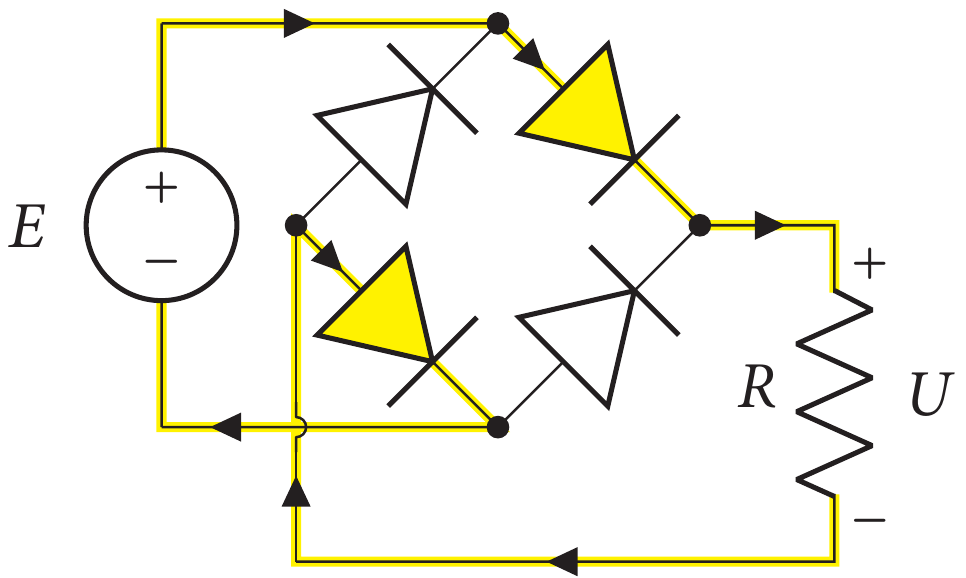
\includegraphics[width=\textwidth]{figures/likriktare_positiv.png}
}

\frame{
\frametitle{}
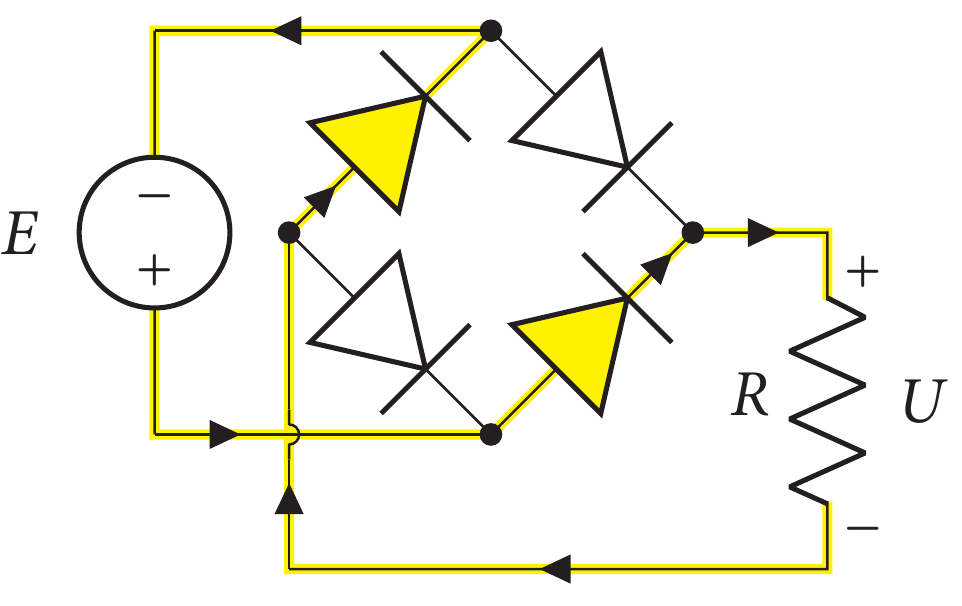
\includegraphics[width=\textwidth]{figures/likriktare_negativ.png}
}

\frame{
\frametitle{}
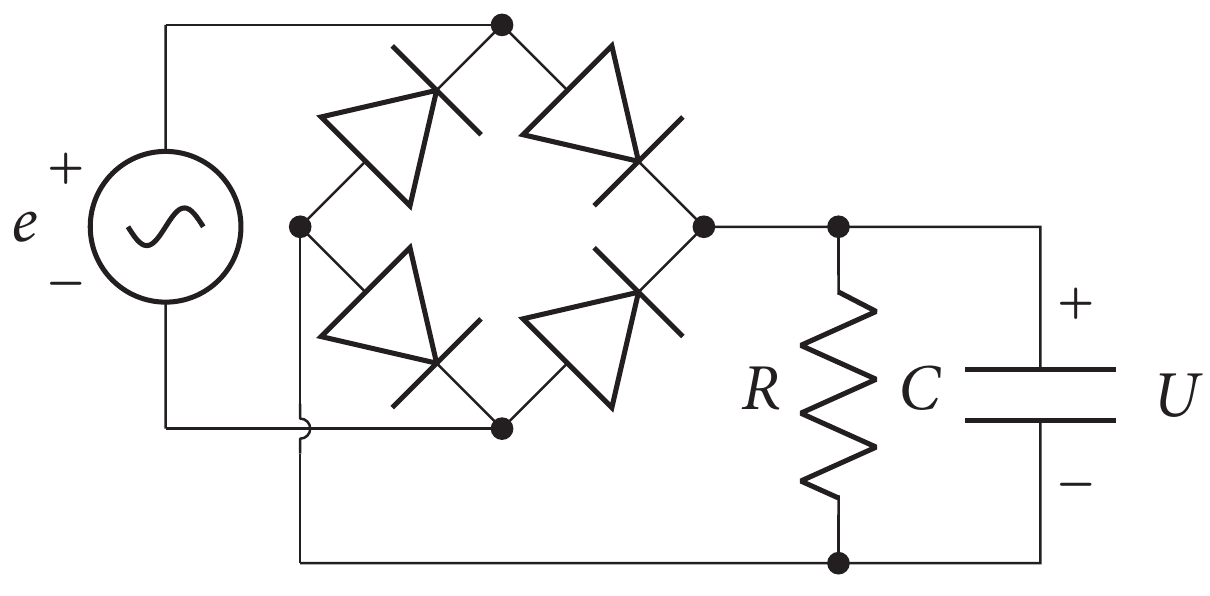
\includegraphics[width=\textwidth]{figures/likriktare_glattad.png}
}

\handoutnoteslide

\mode<beamer>{
\frame{
\frametitle{}\centering
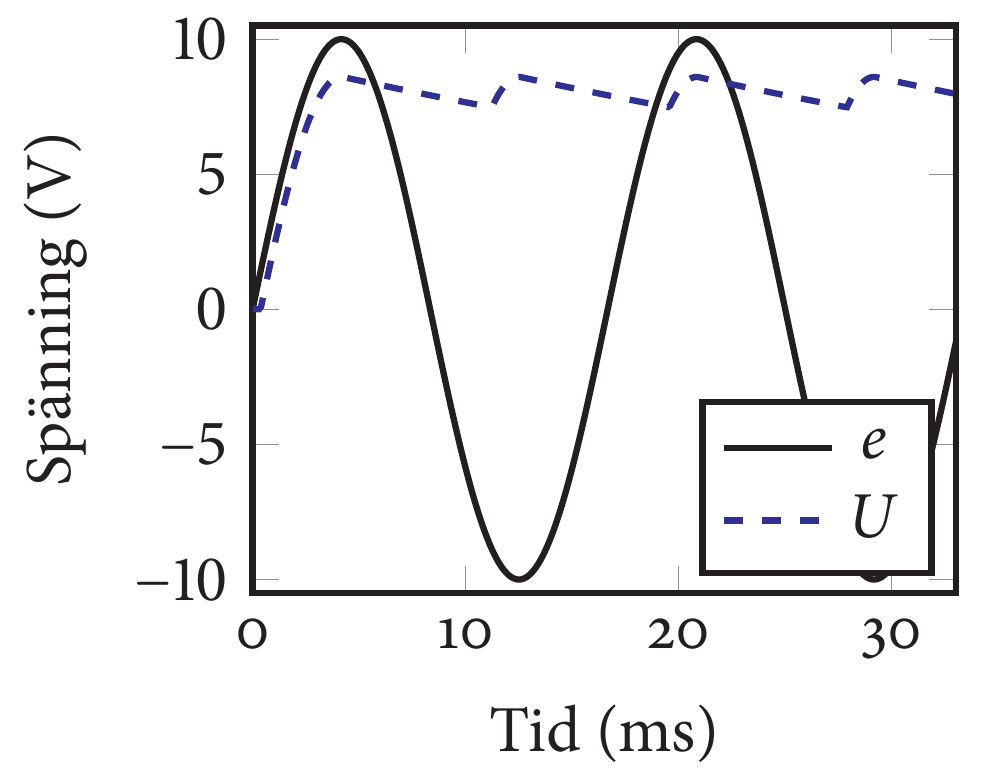
\includegraphics[width=0.7\textwidth]{figures/likriktare_glattad_svaret.png}
}
}

\end{document}
